%!TEX root = ../prueba.tex
En este capítulo se describen los diagramas de secuencia que indican la forma en que los diferentes objetos se comunican entre si para presentar información en la pantalla correspondiente.

\section{SEQ01-Diagrama de Secuencia de Login}
\begin{description}
	\item[Diagrama:]\hspace{1pt}
	\begin{figure}[hbtp!]
		\begin{center}
			\fbox{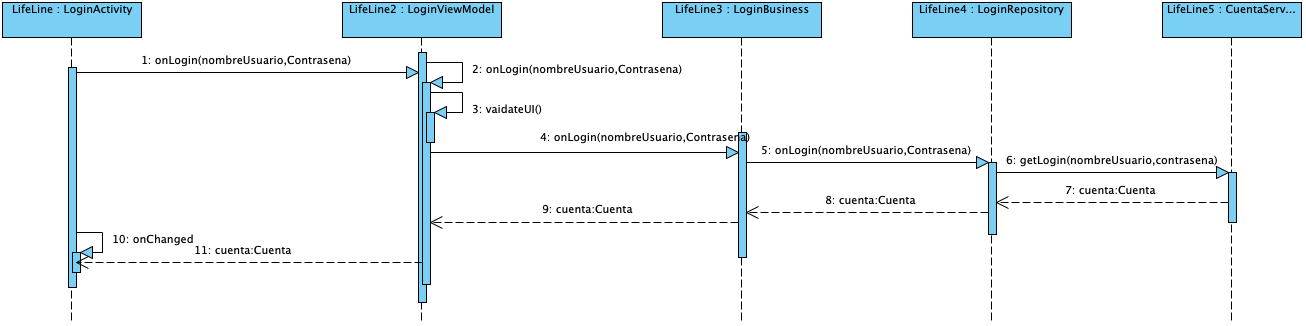
\includegraphics[width=\textwidth]{seq/loginSeq}}
			\caption{Diagrama de Secuencia de Login}
			\label{fig:SEQ01}
		\end{center}
	\end{figure}
	
	\item[Caso de Uso:]\getElementById[CU]{CUMAU1}

\end{description}



\section{SEQ02-Diagrama de Secuencia de Consulta de Locales}

\begin{description} 
	\item[Diagrama:]\hspace{1pt}
	\begin{figure}[hbtp!]
		\begin{center}
			\fbox{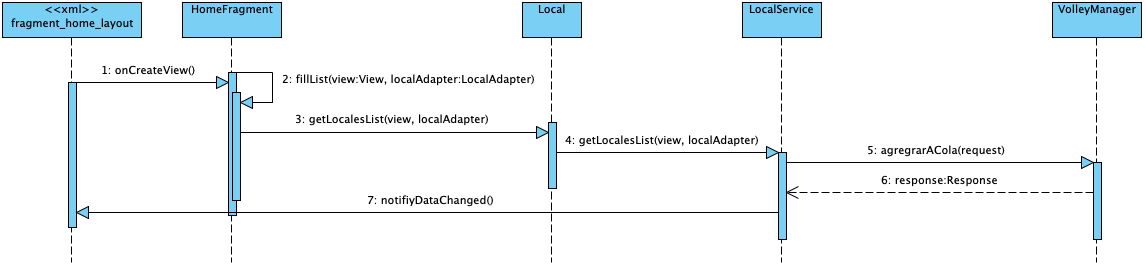
\includegraphics[width=\textwidth]{seq/localesSeq}}
			\caption{Diagrama de Secuencia de Consulta de Locales}
			\label{fig:SEQ02}
		\end{center}
	\end{figure}
	
	\item[Caso de Uso:]\getElementById[CU]{CUMC3}
\end{description}